% 图 5.19 MnO 中子衍射谱 80K/293K
% 谱峰按 lambda=1.06 A, a0(80K)=8.85 A, a0(293K)=4.43 A 的高斯合成重建
% After C. G. Shull, W. A. Strauser and E. O. Wollan, Phys. Rev. 83, 333 (1951)
\documentclass[tikz,border=5pt]{standalone}
\usetikzlibrary{arrows.meta,calc}
\usepackage{amsmath}
\usepackage{bm}
\usepackage{fontspec}
\setmainfont{Times New Roman}
\usepackage{pgfplots}
\pgfplotsset{compat=1.18}
\begin{document}
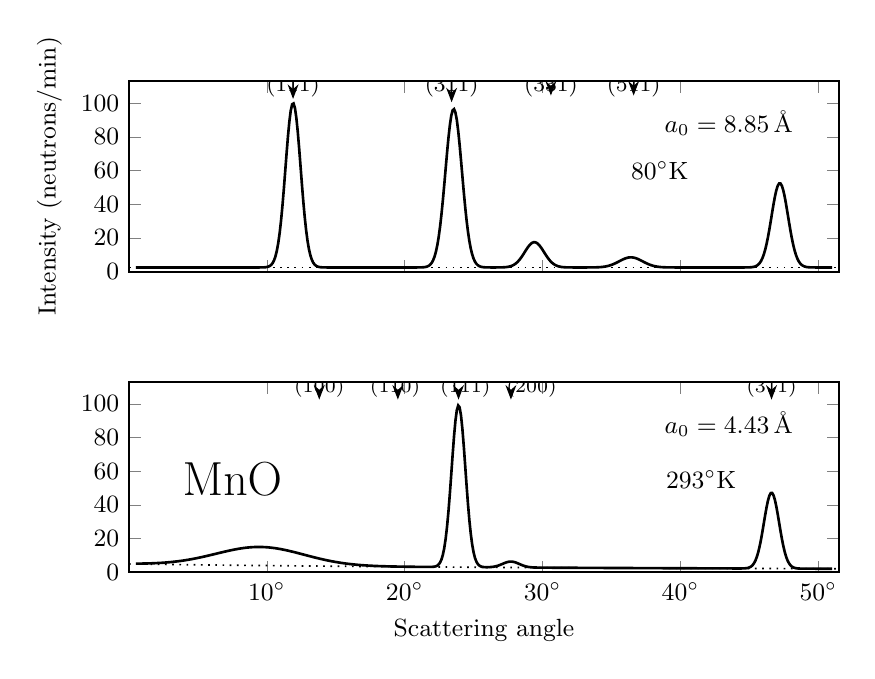
\begin{tikzpicture}[line width=0.8pt,>=Stealth]
\begin{axis}[name=topA,
  at={(0cm,4.0cm)}, anchor=north west,
  width=10.6cm, height=4.0cm,
  xmin=0, xmax=51.5, ymin=0, ymax=113,
  xtick={10,20,30,40,50}, xticklabels={},
  ytick={0,20,40,60,80,100},
  axis line style={line width=0.7},
  tick label style={font=\small},
  label style={font=\small},
  ylabel={Intensity (neutrons/min)},
  trim axis left]
  \addplot[dotted,line width=0.6,domain=0:51.5] {2.5};
  \addplot[line width=0.95,domain=0.5:51,samples=500]
    {2.5 + 97.5*exp(-(x-11.9)^2/(2*0.55^2))
         + 94*exp(-(x-23.55)^2/(2*0.6^2))
         + 15*exp(-(x-29.4)^2/(2*0.7^2))
         + 6*exp(-(x-36.4)^2/(2*0.85^2))
         + 50*exp(-(x-47.2)^2/(2*0.6^2))};
  % magnetic peak indices (80 K, magnetic cell a=8.85 A)
  \node[font=\footnotesize] at (axis cs:11.9,110) {(111)};
  \draw[->,line width=0.5] (axis cs:11.9,108) -- (axis cs:11.9,102.5);
  \node[font=\footnotesize] at (axis cs:23.4,110) {(311)};
  \draw[->,line width=0.5] (axis cs:23.4,108) -- (axis cs:23.4,100.5);
  \node[font=\footnotesize] at (axis cs:30.6,110) {(331)};
  \draw[->,line width=0.5] (axis cs:30.6,108) -- (axis cs:30.6,104.5);
  \node[font=\footnotesize] at (axis cs:36.6,110) {(511)};
  \draw[->,line width=0.5] (axis cs:36.6,108) -- (axis cs:36.6,104.5);
  \node[font=\small] at (axis cs:38.5,60) {$80^\circ$K};
  \node[font=\small] at (axis cs:43.5,88) {$a_0=8.85$\,\AA};
\end{axis}
% index row of chemical-cell fcc positions (100)(110)(111)(200)(311)
\begin{axis}[name=botA,
  at={(topA.below south west)}, anchor=north west, yshift=-0.72cm,
  width=10.6cm, height=4.0cm,
  xmin=0, xmax=51.5, ymin=0, ymax=113,
  xtick={10,20,30,40,50},
  xticklabels={$10^\circ$,$20^\circ$,$30^\circ$,$40^\circ$,$50^\circ$},
  ytick={0,20,40,60,80,100},
  axis line style={line width=0.7},
  tick label style={font=\small},
  label style={font=\small},
  xlabel={Scattering angle},
  trim axis left]
  \addplot[dotted,line width=0.6,domain=0:51.5,samples=60] {1.5+3.5*exp(-x/30)};
  \addplot[line width=0.95,domain=0.5:51,samples=500]
    {1.5+3.5*exp(-x/30)
         + 11*exp(-(x-9.5)^2/(2*3.2^2))
         + 96*exp(-(x-23.9)^2/(2*0.5^2))
         + 3.5*exp(-(x-27.7)^2/(2*0.6^2))
         + 45*exp(-(x-46.6)^2/(2*0.55^2))};
  \node[font=\scriptsize] at (axis cs:13.8,109.5) {(100)};
  \draw[->,line width=0.5] (axis cs:13.8,107.5) -- (axis cs:13.8,102.5);
  \node[font=\scriptsize] at (axis cs:19.3,109.5) {(110)};
  \draw[->,line width=0.5] (axis cs:19.5,107.5) -- (axis cs:19.5,102.5);
  \node[font=\scriptsize] at (axis cs:24.4,109.5) {(111)};
  \draw[->,line width=0.5] (axis cs:23.9,107.5) -- (axis cs:23.9,102.5);
  \node[font=\scriptsize] at (axis cs:29.2,109.5) {(200)};
  \draw[->,line width=0.5] (axis cs:27.7,107.5) -- (axis cs:27.7,102.5);
  \node[font=\scriptsize] at (axis cs:46.6,109.5) {(311)};
  \draw[->,line width=0.5] (axis cs:46.6,107.5) -- (axis cs:46.6,102.5);
  \node[font=\LARGE] at (axis cs:7.5,55) {MnO};
  \node[font=\small] at (axis cs:41.5,55) {$293^\circ$K};
  \node[font=\small] at (axis cs:43.5,88) {$a_0=4.43$\,\AA};
\end{axis}
\end{tikzpicture}
\end{document}
